\begin{center}
    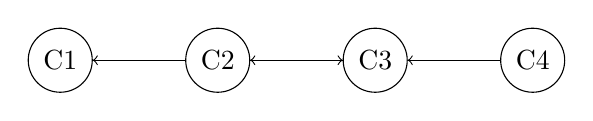
\begin{tikzpicture}[
        node/.style={
            circle, 
            draw,
            radius=1cm,
        }
    ]

    \node (C1) at (0,0) [node] {C1};
    \node (C2) at (2,0) [node] {C2};
    \node (C3) at (4,0) [node] {C3};
    \node (C4) at (6,0) [node] {C4};

    \draw [->] (C2) -- (C1);
    \draw [->] (C3) -- (C2);
    \draw [->] (C2) -- (C3);
    \draw [->] (C4) -- (C3);
    
    

    \end{tikzpicture}
\end{center}